% a jem of a website: https://mpetroff.net/files/beamer-theme-matrix/
\documentclass[xcolor={dvipsnames,svgnames}]{beamer}
\usetheme{PaloAlto}
\usecolortheme{spruce}
\usepackage[utf8]{inputenc}
\usepackage{enumerate}
\usepackage{amsmath}
\usepackage{amsthm}
\usepackage{amssymb}
\usepackage{amsbsy}
\usepackage{amsfonts}
\usepackage{hyperref}
\usepackage{tikz}
\usepackage{verbatim}
\usepackage{mathtools}
\usepackage{macros}
\usepackage{float}
\usepackage{caption}
\usepackage{subcaption}
\usepackage{xcolor,graphicx}
\usepackage{animate}
\usepackage{tikz}
\usetikzlibrary{positioning}
\setbeamertemplate{caption}[numbered]
\DeclareUnicodeCharacter{2212}{-}
\usepackage{tikz-cd}
\usepackage{flowchart}
\usetikzlibrary{
  shapes,
  arrows.meta, % supersedes arrows
  calc,automata,positioning,fit,quotes}
  \tikzset{
  line/.style={draw, -Latex}
}
\tikzstyle{arrow} = [thick,->,>=stealth]
\captionsetup{font=scriptsize,labelfont={bf,sf}}
\captionsetup[subfigure]{font=scriptsize,labelfont=scriptsize}

\makeatletter
  \setbeamertemplate{sidebar \beamer@sidebarside}%{sidebar theme}
  {
    \beamer@tempdim=\beamer@sidebarwidth%
    \advance\beamer@tempdim by -6pt%
    \insertverticalnavigation{\beamer@sidebarwidth}%
    \vfill
    \ifx\beamer@sidebarside\beamer@lefttext%
    \else%
      \usebeamercolor{normal text}%
      \llap{\usebeamertemplate***{navigation symbols}\hskip0.1cm}%
      \vskip2pt%
    \fi%
}%
\title[Functional Neural Circuits in Visual System]{Unsupervised Discovery of Functional Neural Circuits in Visual System}
\author{Liu Zhang\\ Mentors: Prof.~Steven W. Zucker and Dr.~Luciano Dyballa\\ Yale Zucker Lab}

\date{October 12, 2021}
\logo{
\includegraphics[width=.075\textwidth]{YaleNUS_workmark_solid.eps}}
\begin{document}

\begin{frame}
\titlepage
\end{frame}

\section{The Problem}
\begin{frame}{The problem: modeling visual perception}
\begin{itemize}
    \item Primary visual cortex (V1)
    \begin{figure}[H]
            \centering
                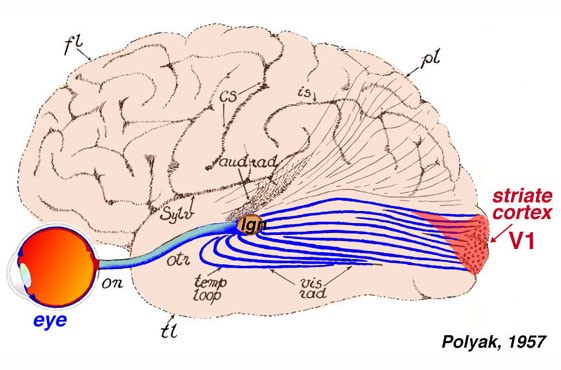
\includegraphics[width=0.25
                \textwidth]{figures-models/v1.jpg}
                \caption{Visual input goes from the eye to primary visual cortex (V1).\\ (Adapted from Polyak (1957))}
            \end{figure}     
        \item How do humans process visual information? 
\end{itemize}
\end{frame}

% \begin{frame}{The bigger picture: Modeling V1}
%     \begin{itemize}
%         \item convolution operator: at simple cells. The convolution of $K(t)$ (e.g. a kernel) and $g(t)$ (e.g. an image), $K \ast g$ is defined by 
%         \begin{align}
%             [K \ast g](t) = \int^t_0 K(u)g(t-u)du.
%         \end{align}
%         \item pooling operator (taking the average or maximum): at complex cells 
%     \end{itemize}  
% \end{frame}

\begin{frame}{Our goals}
       \begin{itemize}
       \item \textit{Functional geometry of neural networks}: the geometric structure arising from how similarly the neurons respond to a given visual stimulus, i.e., how the neurons are organised and connected.
        \item Compare the functional geometry of biological neural networks in the primary visual cortex (V1) and that of artificial neural networks
        \item Models for the primary visual cortex (V1)
    \end{itemize}
\end{frame}

% \begin{frame}{The problem: modeling visual perception}
% \begin{itemize}
%     \item Hierarchy model by Hubel and Wiesel (1965)
%      \begin{figure}[H]
%         \centering
%             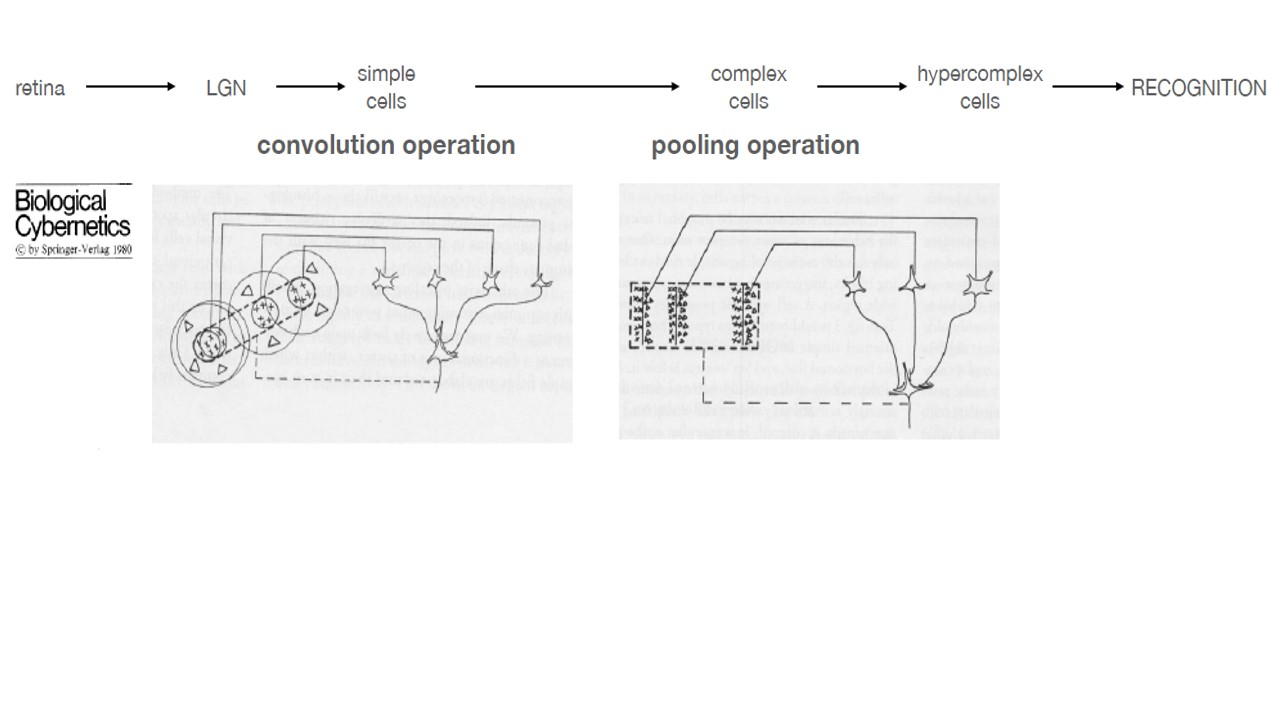
\includegraphics[width=0.8\textwidth]{figures-models/hierarchy-model.jpg}
%             \caption{Hierarchical model of V1. (Adapted from Prof. Zucker's notes)}
%         \end{figure} 
% \end{itemize}
% \end{frame}

\begin{frame}{Data: from lab experiments}
    \begin{itemize}
        \item Visual stimuli of artificial gratings are flashed in front of the mouse.
        \item Neuron output is recorded with electrodes and encoded in peristimulus (PSTH) diagrams.
        \item Each PSTH diagram shows the firing rate of some neuron over time.
    \end{itemize} 
        \begin{minipage}{0.5\textwidth}
    \begin{figure}[H]
        \centering
            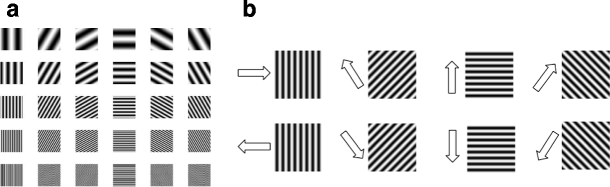
\includegraphics[width=\textwidth]{figures-retina-results/stimuli.png}
            \caption{Visual stimuli: artificial gratings.}
    \end{figure}
    \end{minipage}
    \begin{minipage}{.4\textwidth}  
   \begin{figure}
        \centering
            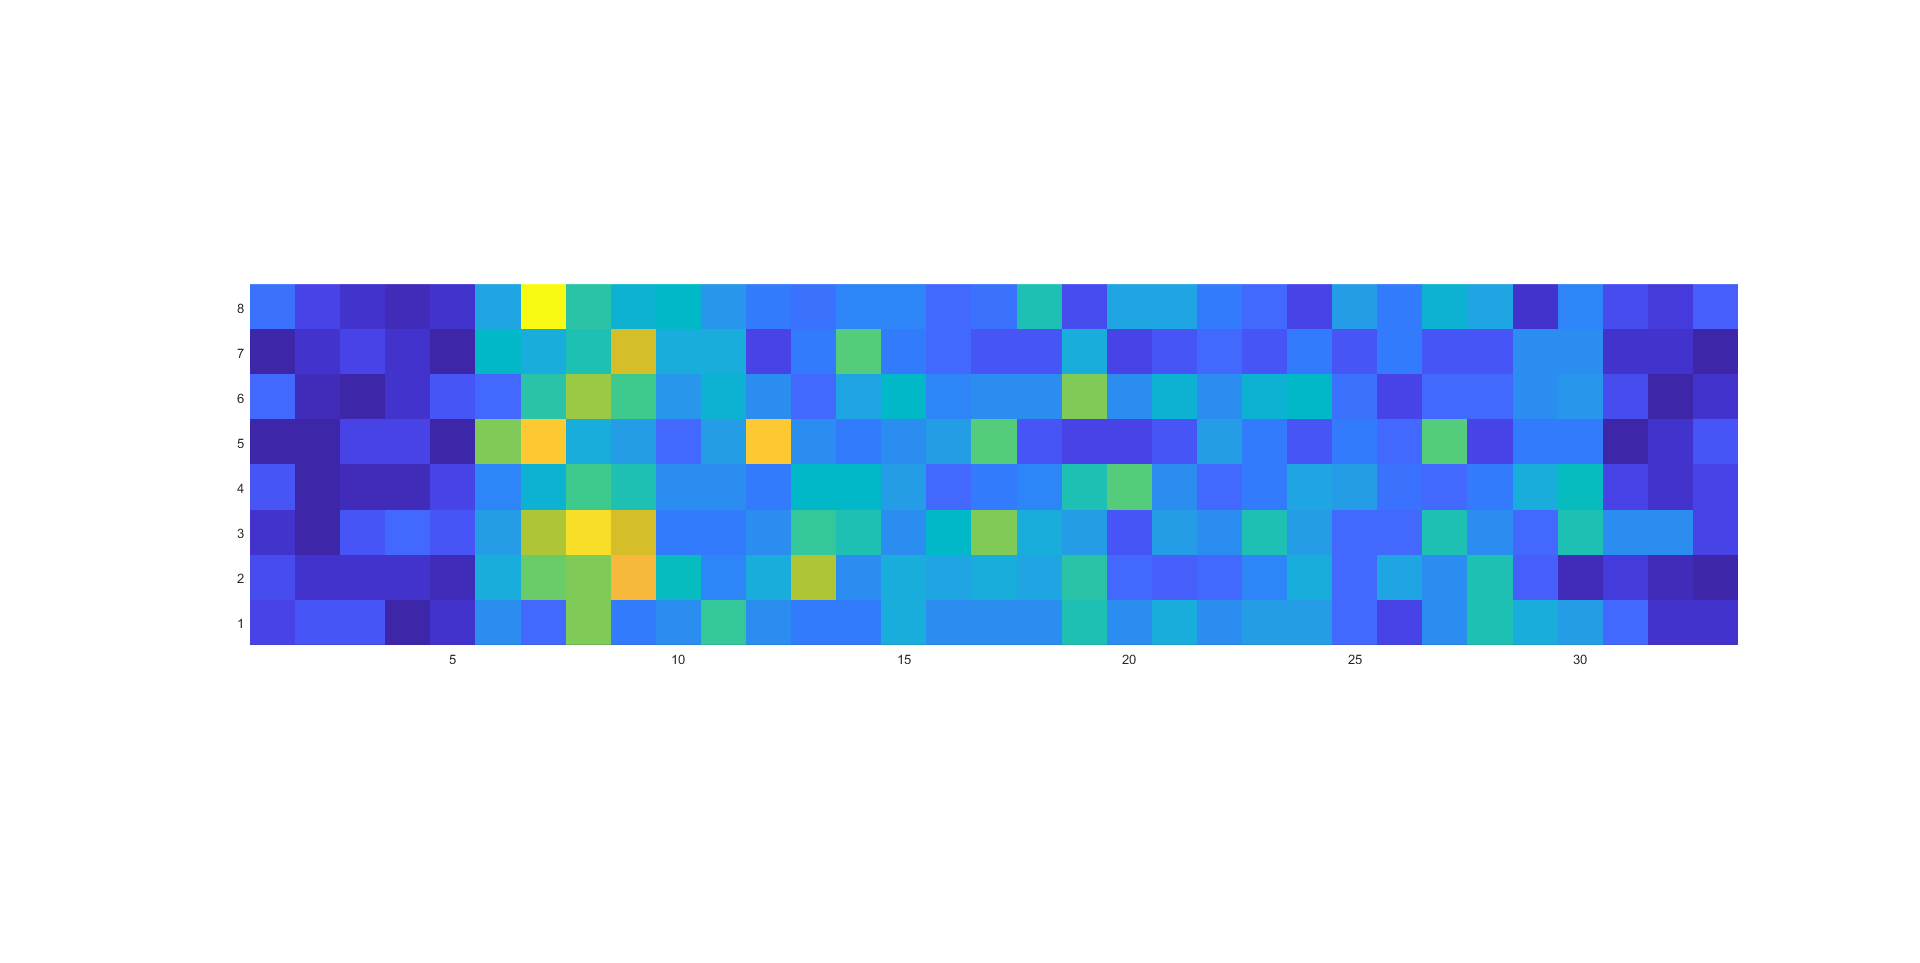
\includegraphics[width=\textwidth]{figures-retina-results/psth.png}
            \caption{Visualising PSTH diagram.}
    \end{figure}
    \end{minipage}%
\end{frame}
\begin{frame}{Data: from computational simulations}
    \begin{itemize}
        \item Input natural images of different objects (e.g. cars, cats, and dogs) to the artificial neural networks (ANNs).
        \item Compute output (numerical values) from neuron units.
    \end{itemize}
    % add image
    \begin{figure}
        \centering
            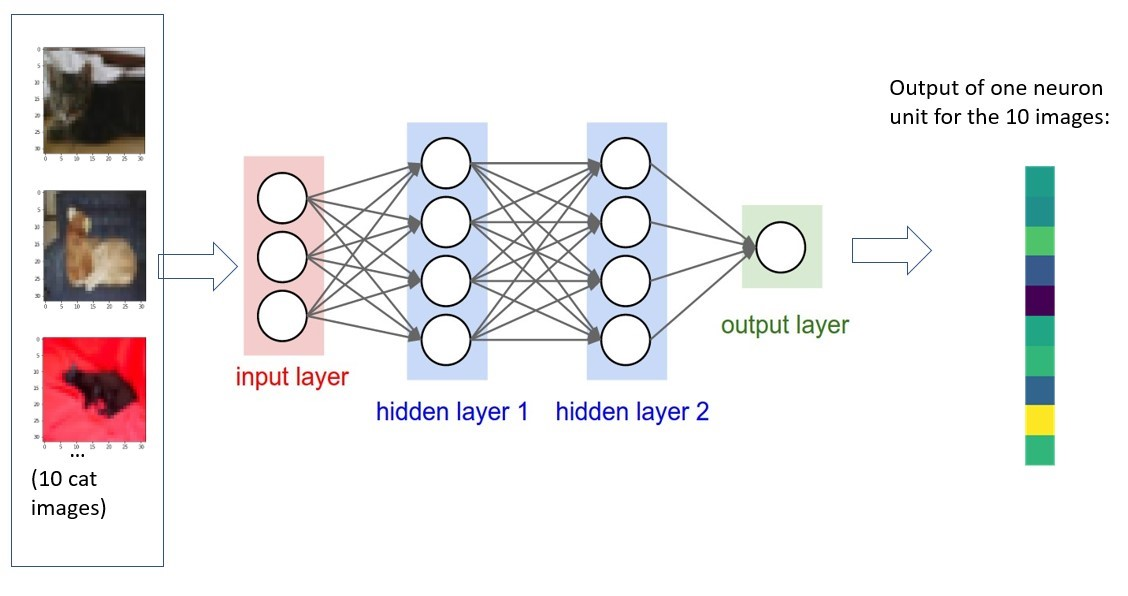
\includegraphics[width=0.9\textwidth]{Slide1.jpg}
            \caption{Computing output of one neuron unit in the ANNs given 10 input cat images.}
    \end{figure}
    % add output
    
\end{frame}

% \begin{frame}{Challenges in neural data analysis in V1}
%     \begin{itemize}
%         \item Limited experimental results\dots
        
%         \item[] Solution: use Artificial Neural Networks (ANNs) to generate artificial neuron tensors.
        
%         \item High-dimensional\dots
        
%       \item[] Solution: use dimensionality reduction methods like tensor factorization and diffusion map. 
        
%         \item Complex geometric structure\dots 
        
%         \item[] Solution: use analytic tools from differential geometry.
%     \end{itemize}
% \end{frame}
\section{The Method}
\begin{frame}{Summary of the method}

 \begin{tikzpicture}[>=latex',font={\sf \small}]
 \def\smbwd{2cm}
 \node (tensors) at (-1,-2) [draw, terminal, minimum width=\smbwd,  fill=red!20, minimum height=0.5cm] {Neuron tensors}; 
 \node (experimental) at (-3,0) [draw, terminal, minimum width=\smbwd,  fill=red!20, minimum height=0.5cm]{neural output (lab)};
  \node (artificial) at (3,-0)[draw, terminal,minimum width=\smbwd,  fill=red!20, minimum height=0.5cm]{neuron output (simulations)};
 \node (TCA) at (-2,-3) [draw, process, minimum width=\smbwd, fill=blue!20, minimum height=0.7cm] {Tensor factorization};
  \node (diffusion) at (2,-3) [draw, process, minimum width=\smbwd, fill=blue!20, minimum height=0.7cm] {Diffusion map};
  \node (manifolds) at (-1,-5) [draw, terminal, minimum width=\smbwd,  fill=green!20, minimum height=0.5cm] {Functional geometry};
 \path [line](tensors) -- (TCA);
  \path [line](tensors) -- (diffusion);
 \path [line](experimental) -- (tensors) ;
 \path [line] (artificial) -- (tensors) ;
  \path [line](diffusion) -- (manifolds);
    \path [line](TCA) -- (manifolds);
 \end{tikzpicture}
\end{frame}
% \section{The Method}
% \begin{frame}{Summary of the method}

%  \begin{tikzpicture}[>=latex',font={\sf \small}]
%  \def\smbwd{2cm}
%  \node (tensors) at (-1,-1.2) [draw, terminal, minimum width=\smbwd,  fill=red!20, minimum height=0.5cm] {Neuron tensors}; 
%  \node (experimental) at (-3,0) [draw, terminal, minimum width=\smbwd,  fill=red!20, minimum height=0.5cm]{neural output (lab)};
%   \node (artificial) at (3,-0)[draw, terminal,minimum width=\smbwd,  fill=red!20, minimum height=0.5cm]{neuron output (simulations)};
%  \node (TCA) at (-1,-2) [draw, process, minimum width=\smbwd, fill=blue!20, minimum height=0.7cm] {Tensor factorization};
%  \node (clusters) at (-1,-3) [draw, terminal, minimum width=\smbwd,  fill=yellow!20, minimum height=0.5cm] {Neurons grouped by similar responses};
%   \node (diffusion) at (-1,-4) [draw, process, minimum width=\smbwd, fill=blue!20, minimum height=0.7cm] {Diffusion map (non-linear dimensionality reduction)};
%   \node (manifolds) at (-1,-5) [draw, terminal, minimum width=\smbwd,  fill=green!20, minimum height=0.5cm] {Manifolds of neurons};
%   \node (coordinates) at (-1,-6) [draw, process, minimum width=\smbwd, fill=blue!20, minimum height=0.7cm] {Analyzing the coordinates and neighborhoods};
%   \node (circuits) at (-1,-7) [draw, terminal, minimum width=\smbwd,  fill=green!20, minimum height=0.5cm] {Local functional circuits};
%   \path [line](tensors) -- (TCA);
%  \path [line](experimental) -- (tensors) ;
%  \path [line] (artificial) -- (tensors) ;
%   \path [line](TCA) -- (clusters);
%   \path [line] (clusters) -- (diffusion);
%   \path [line](diffusion) -- (manifolds);
%   \path [line] (manifolds) -- (coordinates);
%   \path [line] (coordinates) -- (circuits);
%  \end{tikzpicture}
% \end{frame}

% \begin{frame}{Principal Component Analysis (PCA)}

% \begin{itemize}
%     \item PCA is a common linear dimensionality reduction method.
%     \item PCA finds the principal components, i.e., the eigenvectors that correspond to the largest variance.
%     \item The first principal component contain most of the information about the original data. We will not lose too much if we approximate our data by taking just the first few principal components.
% \end{itemize}
% % (With Acrobat reader, an animation of the plots generated during the training process can be viewed below)
% \begin{figure}[H]
% \begin{minipage}[b]{0.8\textwidth}
% \animategraphics[width=\textwidth,loop,autoplay]{8}{pca-animation/frame_}{000}{129}
% \caption{Animation adapted from \cite{pca-se}.}
% \end{minipage}
% \end{figure}  
% \end{frame}

\begin{frame}{From matrices to tensors}
\begin{defn}[Tensors]
    An $N$-way tensor is an element of the tensor product of $N$ vector spaces. 
    \begin{itemize}
        \item $1$-way tensor = vector, $v = [v_1 \quad v_2 \quad \dots \quad v_n]^T.$
        \vfill
        \item $2$-way tensor = matrix, 
        $A = \left(\begin{matrix}
        A_{1 1} & A_{1 2} & \dots & A_{1 n}\\
        \vdots & \vdots & \vdots & \vdots \\ 
        A_{m 1} & A_{m 2} & \dots & A_{m n}
        \end{matrix}
        \right).$
        \vfill
        \item $3$-way tensor of dimension $I$-by-$J$-by-$K$:
    \begin{figure}[H]
    \centering
    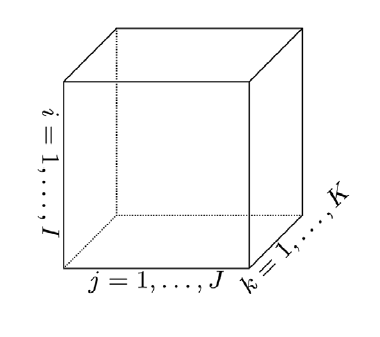
\includegraphics[width=0.35\textwidth]{figures-tensor/tensor-vis.png}
    \end{figure} 
    \end{itemize}
    \end{defn}
\end{frame}

\begin{frame}{From matrix factorization to tensor factorization}
    \begin{figure}[H]
        \centering
            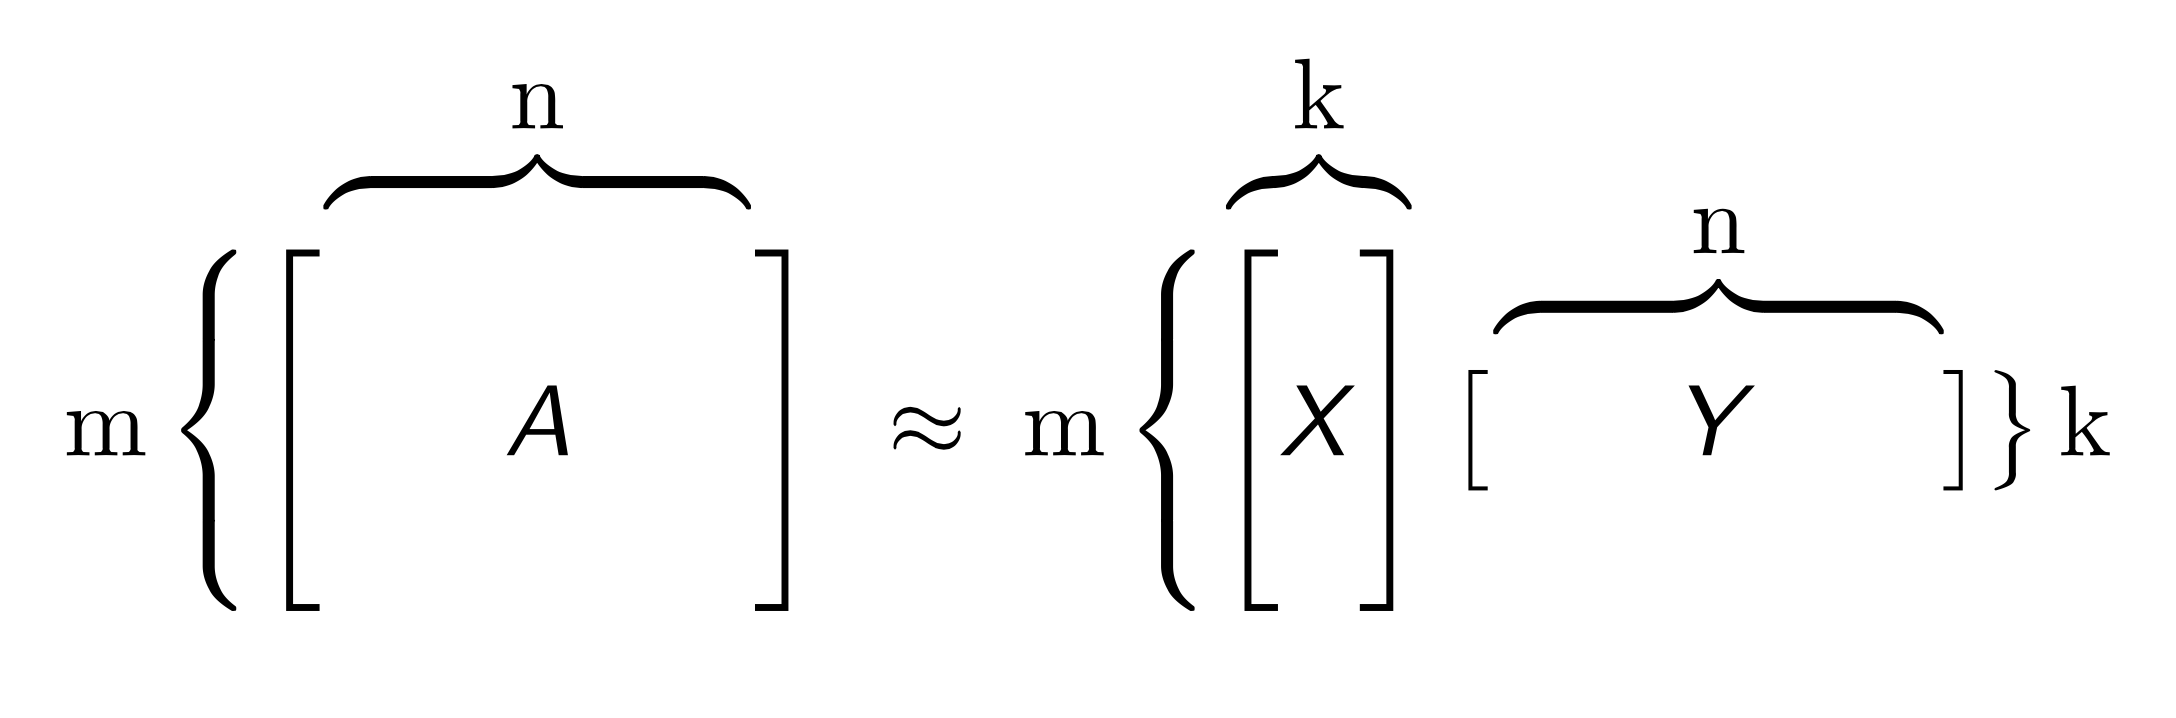
\includegraphics[width=0.8\textwidth]{figures-tensor/matrix_decomp.png}
            \caption{Intuition for matrix factorization.}
        \end{figure} 
    \begin{figure}[H]
        \centering
            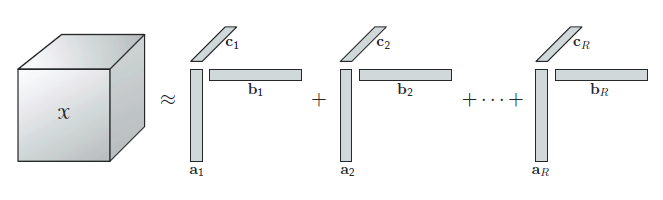
\includegraphics[width=0.8\textwidth]{figures-tensor/cp-decomp.png}
            \caption{Intuition for tensor factorization. (Adapted from \cite{Kol2009}.)}
        \end{figure} 
\end{frame}

\section{The Results}
\begin{frame}{Demo: apply tensor factorization to face image data (from 1000 face images to 5 features)}
\begin{figure}[H]
        \centering
            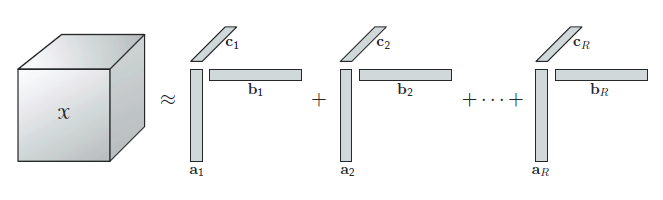
\includegraphics[width=0.8\textwidth]{figures-tensor/cp-decomp.png}
            \caption{Intuition for tensor factorization. (Adapted from \cite{Kol2009}.)}
        \end{figure} 
    \begin{figure}[H]
        \centering
            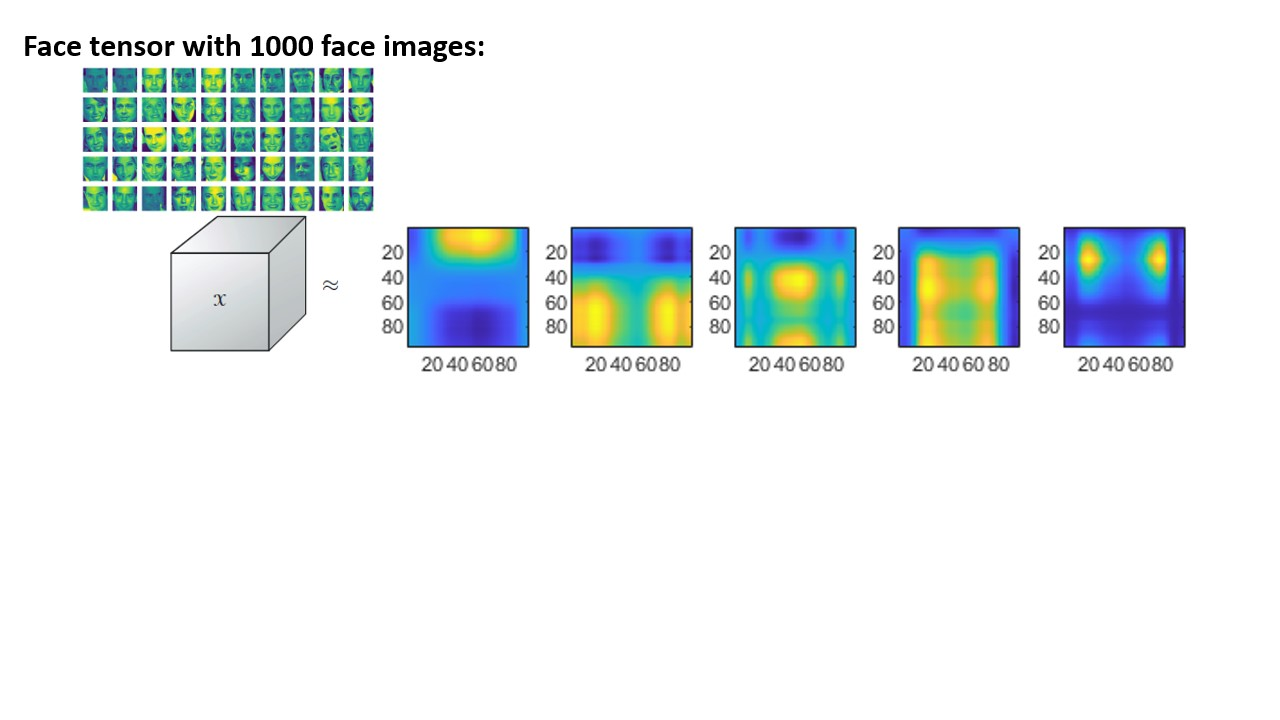
\includegraphics[width=0.9\textwidth]{Slide2.jpg}
            \caption{First 5 tensor factors for face image data.}
        \end{figure} 
\end{frame}

\begin{frame}{Demo: apply tensor factorization to face image data (face images by cluster)}
      \begin{figure}[H]
            \centering
            \begin{subfigure}[b]{0.45\textwidth}
                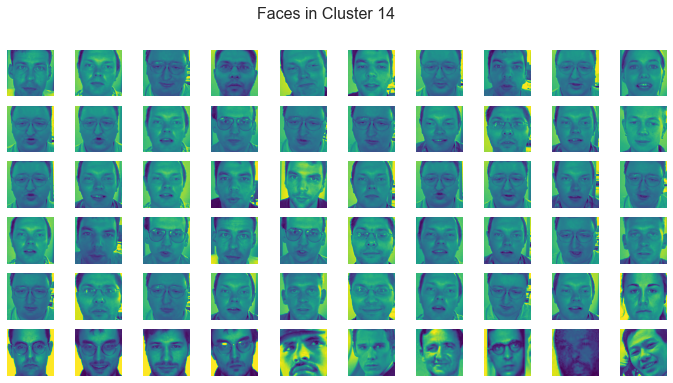
\includegraphics[width=\textwidth]{figures-face-results/face14.png}
            \end{subfigure}
            \hfill 
            \begin{subfigure}[b]{0.45\textwidth}
                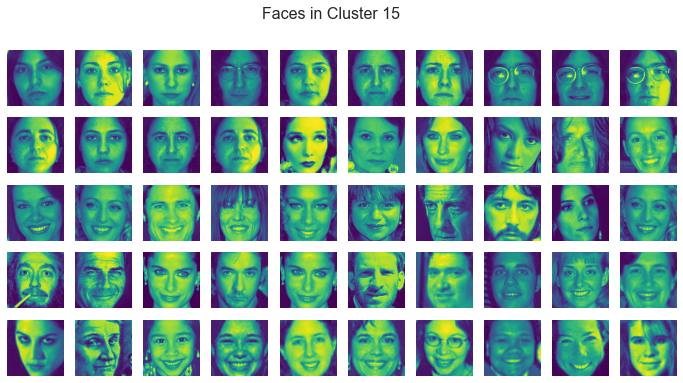
\includegraphics[width=\textwidth]{figures-face-results/face15.png}
            \end{subfigure}
            \hfill
            \begin{subfigure}[b]{0.45\textwidth}
                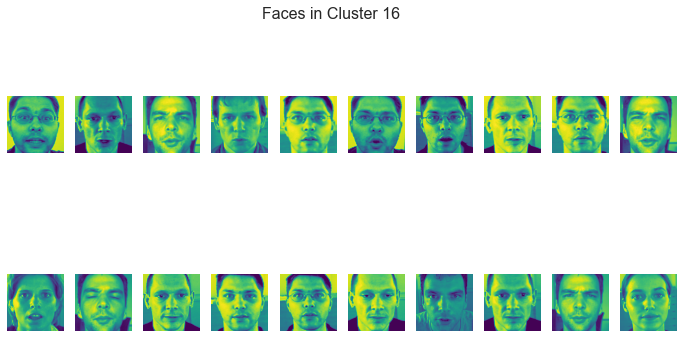
\includegraphics[width=\textwidth]{figures-face-results/face16.png}
            \end{subfigure}
            \hfill
            \begin{subfigure}[b]{0.45\textwidth}
                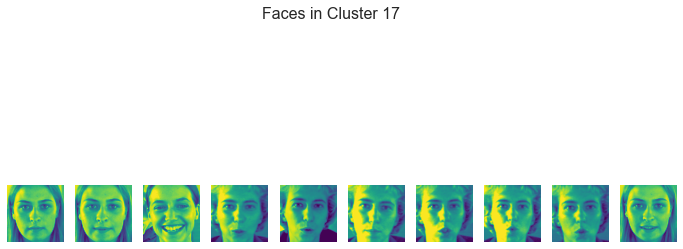
\includegraphics[width=\textwidth]{figures-face-results/face17.png}
            \end{subfigure}
            \caption{Some arbitrary clusters showing the results of TCA for face data.}
            \end{figure} 
\end{frame}

\begin{frame}{Results: apply tensor factorization to retina neural data (from 698 PSTH images to 5 features)}
\begin{figure}[H]
        \centering
            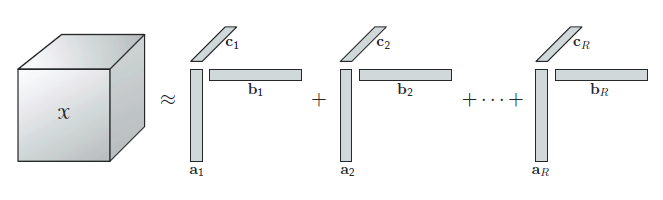
\includegraphics[width=0.8\textwidth]{figures-tensor/cp-decomp.png}
            \caption{Intuition for tensor factorization. (Adapted from \cite{Kol2009}.)}
        \end{figure} 
    \begin{figure}[H]
        \centering
            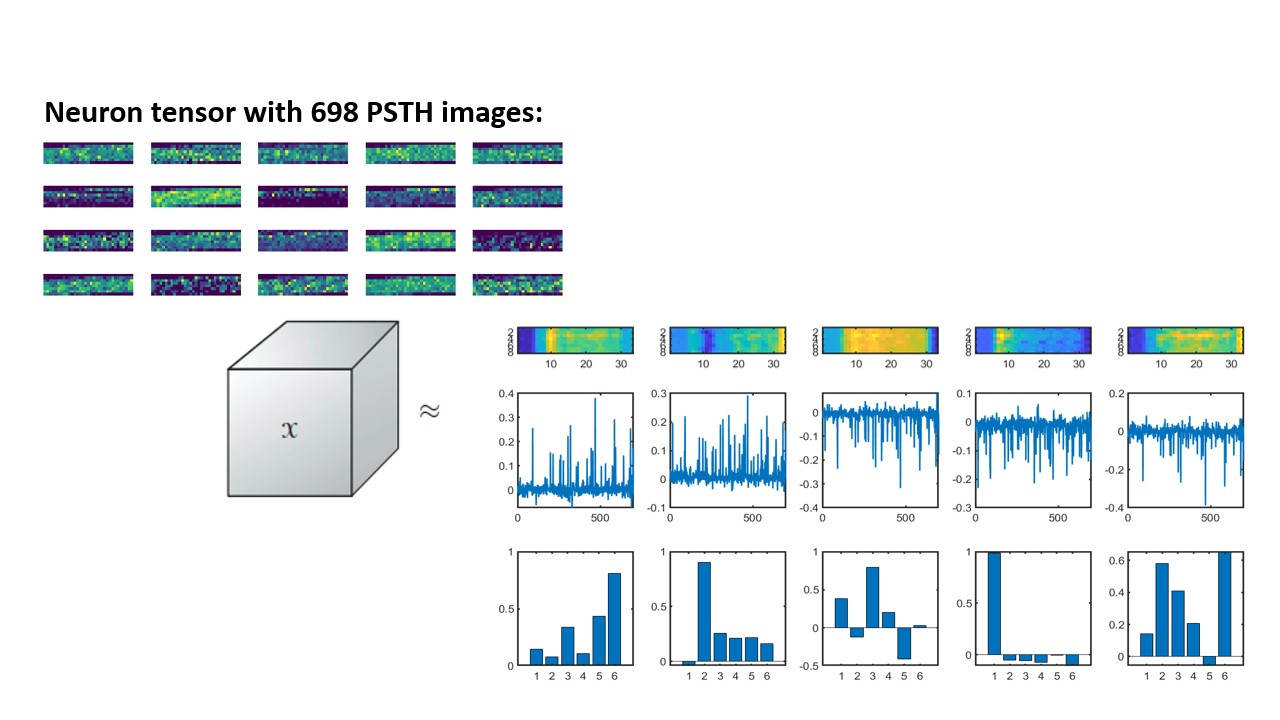
\includegraphics[width=0.9\textwidth]{Slide3.jpg}
            \caption{First 5 tensor factors for neural data.}
        \end{figure} 
        
\end{frame}
\begin{frame}{Results: apply tensor factorization to retina neural data (neuron clusters, i.e., the functional geometry)}
      \begin{figure}[H]
            \centering
            \begin{subfigure}[b]{\textwidth}
                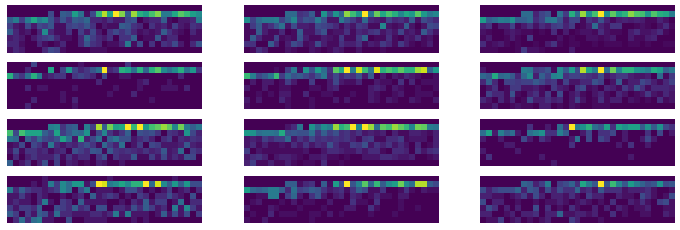
\includegraphics[width=0.95\textwidth]{figures-retina-results/cluster20.png}
                \caption{PSTH diagrams showing responses of neurons within some arbitrary cluster to stimuli of type 1.}
            \end{subfigure}
            \vfill 
            \begin{subfigure}[b]{\textwidth}
                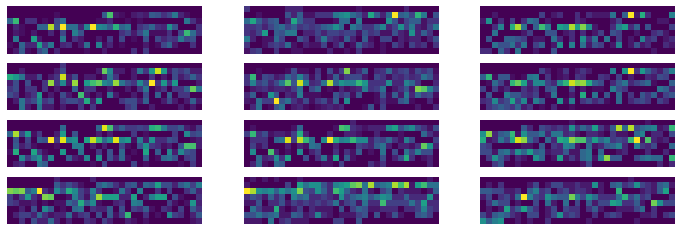
\includegraphics[width=0.95\textwidth]{figures-retina-results/cluster10.png}
                \caption{PSTH diagrams showing responses of neurons within a different cluster to stimuli of type 1.}
            \end{subfigure}
            \end{figure} 
\end{frame}
\begin{frame}{Putting it all together and next steps:}
\begin{figure}[H]
        \centering
            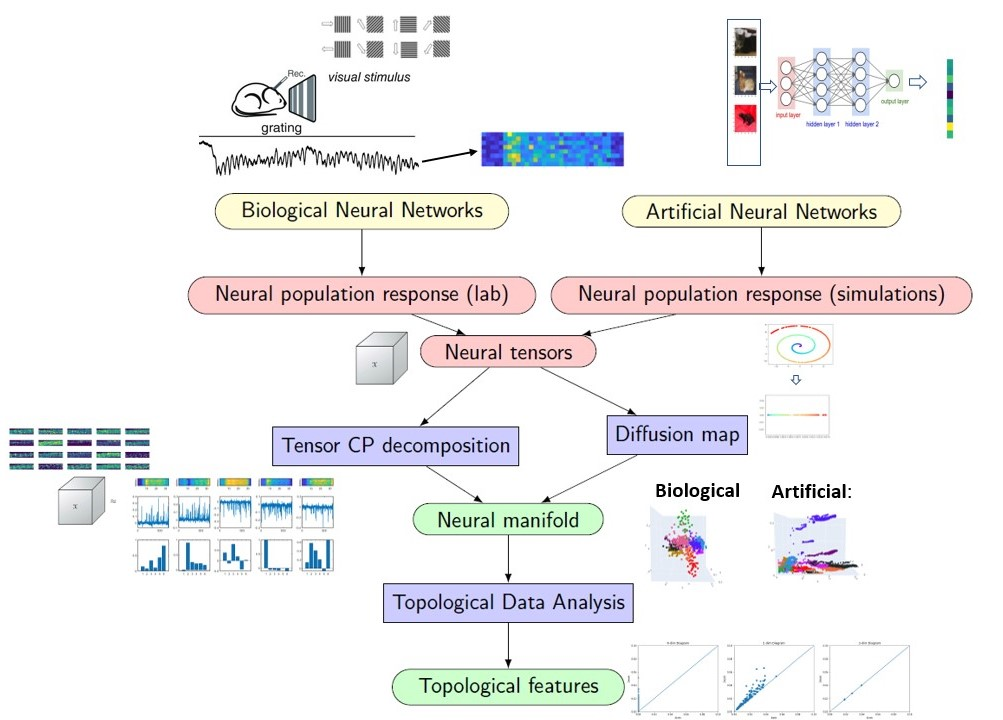
\includegraphics[width=1.2\textwidth]{Slide4.jpg}
        \end{figure} 
\end{frame}

% \begin{frame}{More on convolution and kernels} 

% We can define the kernel and convolve it with an image so as to modify the image in a desired way. For example: 
% \begin{itemize}
%     \item The Gaussian kernel blurs the image:
%     \begin{figure}[H]
%         \centering
%             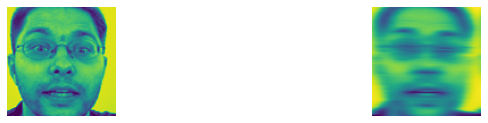
\includegraphics[width=0.8\textwidth]{figures-face-results/face_gaussian.png}
%         \end{figure} 
%     \item The Laplacian of Gaussian kernel sharpens the image:
%     \begin{figure}[H]
%         \centering
%             
\includegraphics[width=0.8\textwidth]{figures-face-results/face_laplacian_overlay.png}
%         \end{figure} 
% \end{itemize}
%     % Note that the ``sharpening" here is not the inverse of ``blurring." We would need a ``deblurring" kernel. 
% \end{frame}

% \begin{frame}{Bonus Slide: Recent Progress}
% For 

% \end{frame}
% \begin{frame}{Alternative to the hierarchy model: recurrent models}
% \textbf{Recurrent models: study networks of cortical connections instead of individual cells. }

% Recurrent computation: 
% \begin{align}
%     S_i(\lambda) = \sum_{j \in \text{neigh}(i)}\sum_{\lambda^\prime \in \Lambda(j)} r_{i,j}(\lambda, \lambda^\prime) p_j(\lambda^\prime)\\
%     P^{t+1}_i(\lambda) = \prod_k [P_i^t(\lambda) + \delta s_i(\lambda)]
% \end{align}

%     \begin{figure}[H]
%     \begin{subfigure}{0.45\textwidth}
%       \centering
%       \subfloat[]{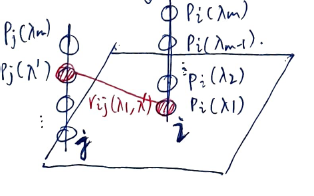
\includegraphics[width=2in]{figures-models/cortical2.png}}
%     \end{subfigure}
%     \hfill
%     \begin{subfigure}{0.45\textwidth}
%       \centering
%       \subfloat[]{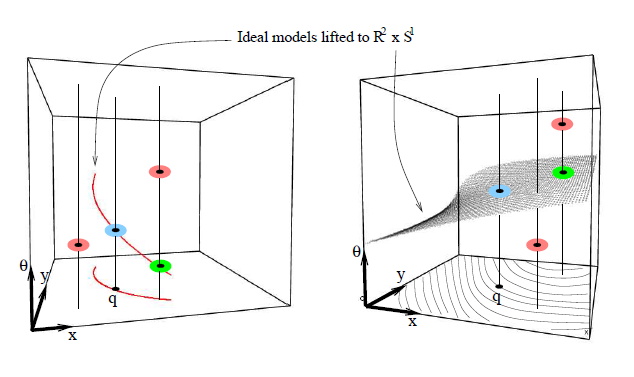
\includegraphics[width=2in]{figures-models/cortical1.png}}
%     \end{subfigure}
%     \end{figure}
% \end{frame}

% \begin{frame}{Bonus slide: modeling lateral inhibition}
% Algebraic model for lateral inhibition: 
% \begin{align}
%     F_i = e_i - \sum_{j \in \text{neighbors}(i)}\alpha_{i,j} \quad e_j, \quad \alpha_{i,j} \in \mathbb{R}^{+}.
% \end{align}
%     \begin{figure}[H]
%         \centering
%             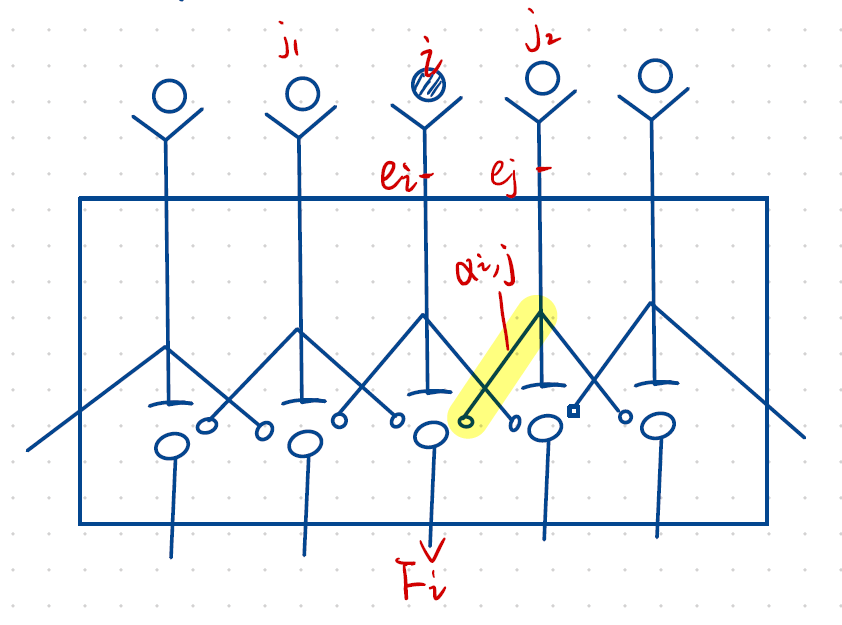
\includegraphics[width=0.7\textwidth]{figures-models/lateral-inhibition.png}
%         \end{figure} 
% \end{frame}

\begin{frame}{Acknowledgements}
    I would like to thank my mentors Prof.~Steven W. Zucker and Dr.~Luciano Dyballa for their generous guidance and advice. They have made possible the many serendipitous moments in this project. I am also grateful for Yale-NUS CIPE for their general support and for my advisor Prof.~Francesca Spagnuolo for her encouragement throughout my mathematical career.
\end{frame}

\section{References}
\begin{frame}{References}
\bibliographystyle{plain}
\bibliography{refs}
\end{frame}

\end{document}